\documentclass[11pt,a4paper]{article}
\usepackage[utf8]{inputenc}
\usepackage[english]{babel}
\usepackage{amsmath}
\usepackage{amsfonts}
\usepackage{amssymb}
\usepackage{graphicx}
\usepackage{listings}
\usepackage{xcolor}
\usepackage{geometry}
\usepackage{booktabs}

\geometry{margin=1in}

% Code snippet styling - FIXED TYPO HERE (\lstdefinestyle)
\definecolor{codegreen}{rgb}{0,0.6,0}
\definecolor{codegray}{rgb}{0.5,0.5,0.5}
\definecolor{codeblue}{rgb}{0.1,0.2,0.8}
\definecolor{backcolour}{rgb}{0.96,0.96,0.98}

\lstdefinestyle{mystyle}{
    backgroundcolor=\color{backcolour},   
    commentstyle=\color{codegreen},
    keywordstyle=\color{codeblue},
    numberstyle=\tiny\color{codegray},
    stringstyle=\color{purple},
    basicstyle=\ttfamily\footnotesize,
    breakatwhitespace=false,         
    breaklines=true,                 
    captionpos=b,                    
    keepspaces=true,                 
    numbers=left,                    
    numbersep=5pt,                  
    showspaces=false,                
    showstringspaces=false,
    showtabs=false,                  
    tabsize=4,
    frame=single,
    rulecolor=\color{lightgray}
}
\lstset{style=mystyle}

\title{\textbf{Technical Report: Object-Centric Bimanual Coordinated Control}}
\author{Luca Morello}
\date{\today}

\begin{document}

\maketitle

\begin{abstract}
This report outlines the mathematical reformulation, and control architecture for a bimanual coordinated manipulation system within the \texttt{mc\_rtc} framework. 
\end{abstract}

\section{System Architecture (Object-Centric Control)}
Instead of a master and follower arm,connected by a virstual and spring and damper, the system adopts a \textbf{object-centric approach}. A virtual object reference frame, denoted as $X_{0,\text{object}}$, is defined and dynamically tracked relative to the global world frame ($0$).

\subsection{Code Framework}
% FIXED FLOAT SPECIFIER HERE TO [htbp]
\begin{figure}[htbp]
\centering
\small
\begin{verbatim}
       [ IDLE State ]
              |
              | (changeFrame() Triggered)
              v
     [ NEW TARGET GIVEN ]
              |
              v
    [ INDEPENDENT Phase ] ---> Left / Right EndEffectorTasks active
              |
              | (Object Reached: eval().norm() < 0.01)
              v
       [ DUAL Phase ]    ---> Compute Virtual Object Frame & Offsets
              |               Apply leftOffset_ / rightOffset_
              |               left/rightAdmittanceTask_ active
              |
              | (Object Placed at Target Waypoint)
              v
    [ INDEPENDENT Phase ] ---> Re-engage independent arm tasks
\end{verbatim}
\caption{State machine pipeline for collaborative bimanual placement.}
\label{fig:pipeline}
\end{figure}

\subsection{Object Frame Initialization}
The initial virtual object pose is calculated based on the geometric midpoint between the left ($L$) and right ($R$) end-effectors.

\begin{equation}
p_{0,\text{object}} = \frac{p_{0,L} + p_{0,R}}{2}
\end{equation}

\begin{equation}
R_{0,\text{object}} = R_{0,\text{base}}
\end{equation}


% FIXED FLOAT SPECIFIER HERE TO [htbp]
\begin{figure}[htbp]
\centering
\small
\begin{verbatim}
                    [ New Object Position ]
                               |
                +--------------+--------------+
                |                             |
       (Apply leftOffset)            (Apply rightOffset)
                |                             |
                v                             v
     [ Left Hand Target ]          [ Right Hand Target ]
                |                             |
                v                             v
       leftAdmittanceTask_           rightAdmittanceTask_
                |                             |
                v                             v
          Robot Joints 0                Robot Joints 2
\end{verbatim}
\caption{Data flow architecture of the dual-arm object tracking loop.}
\label{fig:architecture}
\end{figure}

\begin{figure}[htbp]
    \centering
    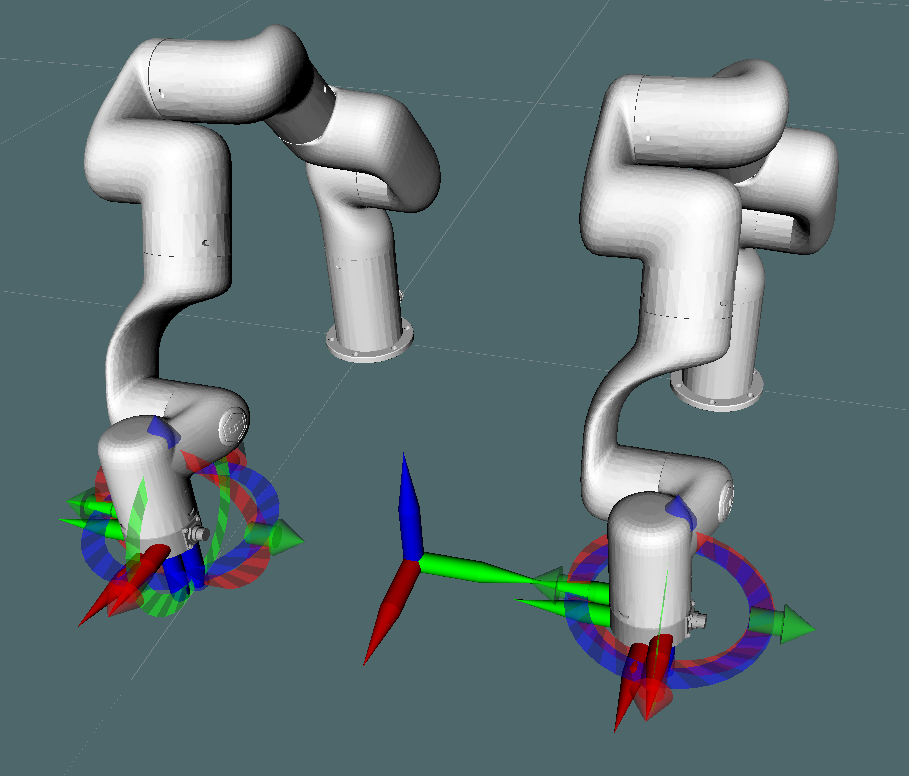
\includegraphics[width=0.5\textwidth]{Images/Dual.png}
    \caption{RVIZ simulation}
    \label{fig:your_figure_label}
\end{figure}




\section{Geometric Invariance via Relative Transformations}
The grasp geometry is frozen at the activation time ($t_0$) by computing the relative transformations (offsets) of the end-effectors with respect to the virtual object frame:

\begin{equation}
X_{\text{object},L} = X_{0, L} \cdot X_{0,\text{object}}^{-1}
\end{equation}
\begin{equation}
X_{\text{object},R} = X_{0, R} \cdot X_{0,\text{object}}^{-1}
\end{equation}

These offsets ($X_{\text{object},L}$, $X_{\text{object},R}$) remain \textbf{strictly constant} throughout the entire manipulation task.

When the target object pose is commanded to follow a trajectory $X_{0,\text{object}}(t)$ over time, the global kinematic targets for the individual end-effectors are updated at each control loop.

\begin{equation}
X_{0,L}^{\text{target}}(t) = X_{\text{object}, L} \cdot X_{0,\text{object}}(t)
\end{equation}
\begin{equation}
X_{0,R}^{\text{target}}(t) = X_{\text{object}, R} \cdot X_{0,\text{object}}(t)
\end{equation}



\section{Rationale and Key Advantages}
\begin{enumerate}
    \item \textbf{Stripped-Down Motion Planning Complexity:} By abstracting the bimanual system into a single virtual operational space.
    \item \textbf{Perfect Geometric Cohesion:} Because the spatial transformations ($X_{\text{object},L}$, $X_{\text{object},R}$) are structurally invariant over time, both arms maintain an identical relative distance and orientation. 
    \item \textbf{Compliance and Tolerance Adaptation via Admittance:} \textbf{To check} the dual admittance tasks seamlessly absorb the error. 
\end{enumerate}


\newpage

\end{document}